\apendice{Especificación de Requisitos}

\section{Introducción}

En esta sección se definen los requisitos de la aplicación así como los objetivos de una forma más esquemática y concreta que en otros apartados. De esta manera se puede ver en que dirección va orientado el proyecto y por qué se ha elegido cada uno de acuerdo a los requisitos.

\section{Objetivos generales}

Estos han sido los principales objetivos del proyecto según la línea de tiempo. Primero creamos un prototipo cliente-servidor para ir conociendo el funcionamiento y una vez entendido, pasar a construir la aplicación con la definición de la gramática. En la construcción de la aplicación se necesita haber entendido el prototipo porque ya ahí se aplica la funcionalidad del cliente y del servidor. Más tarde se van incluyendo los algoritmos sobre las gramáticas formales. Por último, una vez se ha construido la parte esencial de la aplicación podemos centrarnos en crear un registro e inicio de sesión de usuarios.

\subsection{Crear un prototipo de aplicación cliente-servidor con GWT}

El objetivo de crearlo es el de poder ver el funcionamiento, comunicación y procesado del lenguaje Java en GWT para definir que limitaciones y posibilidades de un proyecto realizado con esta herramienta. Con ello se define que:  
\begin{itemize}
\item El lado del cliente y el compartido (shared) son los que se traducen al lenguaje JavaScript y los ficheros se crean dentro de un directorio <<war>>.
\item El lado del cliente tiene ciertas limitaciones y no acepta todo tipo de librerías de Java. 
\item La comunicación entre cliente y servidor es por medio de llamadas de procedimiento remoto o RPC.
\item Parte de la aplicación debe ir indudablemente en el servidor y comunicarse con el cliente para mostrar los resultados.
\end{itemize}

Este primer objetivo es fundamental y marca las posibilidades reales que ofrece GWT de cara a este proyecto.

\subsection{Construir la aplicación con la definición de gramática}

Consiste en hacer ya el comienzo de la aplicación empezando por la <<definición de gramática>> que es la parte de Thoth en la que se introduce una gramática en un campo de texto y el programa es capaz de identificarla y mostrar sus propiedades. Para ello es necesario haber logrado en objetivo anteriormente descrito, ya que se necesita alojar en el servidor el <<parser>> de la gramática y hacerle peticiones desde el cliente para interpretarla y mostrar sus propiedades.

Es el comienzo de la aplicación y la base sobre la que trabajar posteriormente, ya que para implementar los algoritmos es necesario tener definida una gramática.

\subsection{Construir los algoritmos sobre gramáticas}

El objetivo es implementar cada uno de los algoritmos que se aplican sobre una gramática en Thoth. Es una de las utilidades más importantes de esta aplicación y la cual otorga mas posibilidades a los usuarios. Esta compuesta por los algoritmos siguientes:

\begin{itemize}
\item Eliminación de símbolos no terminales.
\item Eliminación de símbolos no alcanzables. 
\item Eliminación de símbolos anulables.
\item Eliminación de producciones no generativas.
\item Eliminación de recursividad directa.
\item Eliminación de recursividad indirecta.
\item Factorización por la izquierda.
\item Forma normal de Chomsky.
\item Análisis descendente LL(K) formado por el cálculo de <<First y Follow>> y reconocimiento por medio de TASP o Tabla de Análisis Sintáctico Predictivo.
\end{itemize}

Hay además dos funcionalidades que engloban varios de estos algoritmos como son la de limpiar gramática y eliminar recursividad.

Varios de ellos tienen la particularidad de que su ejecución esta hecha paso a paso, señalando dichos pasos con un resaltado con colores.

\subsection{Construir un registro de usuarios}

Como la prioridad principal es llevar Thoth a la web y que funcionase correctamente, hacer el registro de usuarios es el objetivo que se encuentra en la última posición. Forma parte de las mejoras con respecto a las anteriores versiones de Thoth, ya que ninguna con esta funcionalidad. Aprovechando la ventaja de que GWT trabaja con comunicación cliente-servidor, decidimos hacer una base de datos en la que registramos los usuarios de la aplicación así como parte de su actividad en Thoth.

Con ello se podrá saber el uso que se le da al proyecto o si los usuarios son activos mostrando, por ejemplo, la hora del último acceso de un usuario o si es utilizado por muchas personas, entre otras ideas. Se debe comprobar que los datos introducidos en el momento de registro, cumplen una serie de requisitos. Además se pretende hacer inicio de sesión para que en caso de que salga de la aplicación, no necesite volver a iniciar el proceso de <<login>>. De esta forma queremos que el usuario se sienta cómodo al utilizar Thoth.
\section{Catálogo de requisitos}

El proceso de realización del proyecto ha requerido de los siguientes pasos:

\begin{itemize}
\item Crear un prototipo de aplicación cliente-servidor con GWT

	\begin{itemize}
	\item Construir la parte del cliente.
	\item Construir la parte del servidor. 
	\item Realizar comunicación entre ambas vía RPC.
	\end{itemize}

\item Construir la aplicación con la definición de gramática
	\begin{itemize}
	\item Construir una vista principal para editar un texto.
	\item Realizar peticiones al servidor. 
	\item Parsear el texto y convertirlo en una gramática.
	\item Devolver la gramática al cliente.
	\item Trabajar con la gramática en el lado del cliente.
	\end{itemize}
\item Construir los algoritmos sobre gramáticas
	\begin{itemize}
	\item Construir cada una de las vistas de los algoritmos.
	\item Trabajar con la gramática recibida y realizar el algoritmo.
	\item Resaltar los pasos realizados por el algoritmo gracias al manejo del texto por medio del lenguaje HTML.
	\item Devolver el resultado a la vista principal en caso de éxito.
	\end{itemize}
\item Construir un registro de usuarios
	\begin{itemize}
	\item Construir un módulo nuevo.
	\item Establecer el cambio entre módulos de forma correcta.
	\item Crear una clase en el servidor que se comunique con el módulo y el cliente.
	\item Registrar información en una base de datos.
	\item Comprobar identificación de un usuario.
	\item Manejar la información del usuario.
	\item Establecer una sesión.
	\end{itemize}
\end{itemize}
\section{Especificación de requisitos}

A continuación, en este apartado se enumeran los casos de uso con una breve descripción de cada uno de ellos.

\begin{itemize}

\item Registro de usuario: Registra los datos de un nuevo usuario.
\item Inicio de sesión: Permite el acceso de un usuario a la aplicación.
\item Cierre de sesión: Aborta la sesión actual del usuario.
\item Crear gramática: Posibilita la creación de una gramática.
\item Modificar gramática: Sirve para realizar cambios sobre la gramática.
\item Algoritmos: Aporta los algoritmos propios de la gramática.
\item Idioma: Cambia el idioma de los textos de la aplicación.
\item Ayuda: Muestra información sobre la aplicación.
\item Renombrar símbolo: Busca un símbolo para después reemplazarlo por otro en una gramática.
\item Comprobar gramática: Comprueba una gramática según una sintaxis definida.
\item Eliminar símbolos no terminales: Suprime los símbolos no terminables de una gramática.
\item Eliminar símbolos no alcanzables: Suprime los símbolos no alcanzables de una gramática.
\item Eliminar símbolos anulables: Quita los símbolos que son anulables de una gramática.
\item Eliminar producciones no generativas: Quita las producciones no generativas de una gramática.
\item Limpiar gramática: Por orden realiza los siguientes algoritmos:
\begin{itemize}
	\item Eliminar símbolos anulables.
	\item Eliminar símbolos no terminables.
	\item Eliminar símbolos no alcanzables.
	\item Eliminar producciones no generativas.
\end{itemize}
\item Eliminar recursividad directa: Suprime la recursividad directa de todas las producciones recursivas.
\item Eliminar recursividad indirecta: Suprime la recursividad indirecta de todas las producciones.

\item Eliminar recursividad: sigue los siguientes pasos
\begin{itemize}
	\item Eliminar recursividad directa.
	\item Eliminar recursividad indirecta.
\end{itemize}

\item Factorizar por la izquierda: Consiste en obtener el prefijo común del
consecuente en todas las producciones que tengan el mismo antecedente,
agrupar esas gramáticas al identificar su prefijo común.
\item Forma normal de Chomsky: consiste en transformar la gramática de forma
que en el consecuente solo aparezca o bien un terminal o bien dos no
terminales.
\item Calculo Firts Follow: Genera las tablas de First y Follow de una gramática.
\item Reconocimiento TASP: Genera la Tabla de Analisis Sintático Predictivo de una gramática y permite comprobar si una palabra es reconocida o no por la gramática
\end{itemize}

\subsection{Diagrama de casos de uso}

Como hay bastantes casos de uso, se utilizarán varios diagramas para documentarlo. Primero se muestra un diagrama del caso de uso general de la aplicación \ref{fig:B.1}. Posteriormente el diagrama \ref{fig:B.2} muestra los casos de uso de crear y modificar una gramática.

\begin{figure}[h]
\centering
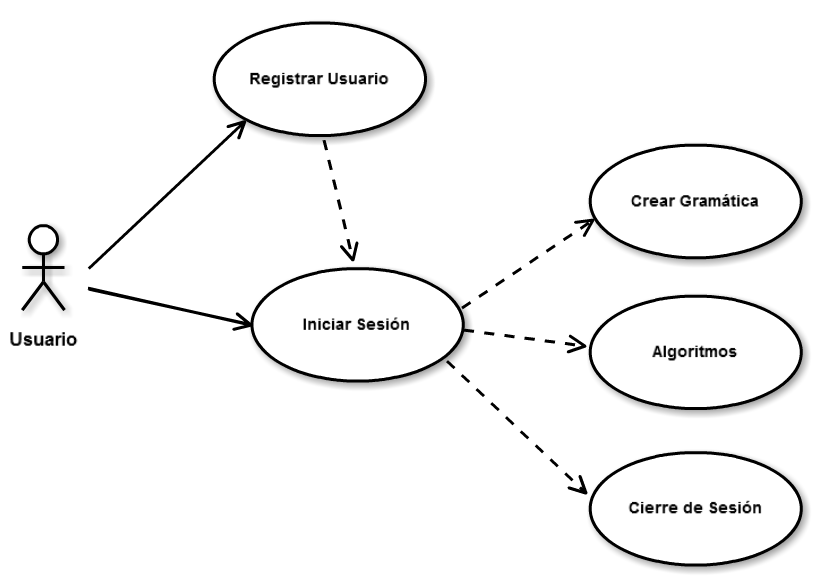
\includegraphics[width=.7\textwidth]{CasoUso-General}
\caption{Diagrama de caso de uso general.}
\label{fig:B.1}
\end{figure}


\begin{table}[]
\centering

\begin{tabular}{@{}
>{\columncolor[HTML]{FFFFFF}}p {.25\textwidth} p {.75\textwidth}@{}}
\toprule
\textbf{Caso de uso 1}   & Registrar un nuevo usuario.                                                                                                                                                                                                                                                                                                                                                          \\ \midrule
\textbf{Versión}         & 1.0                                                                                                                                                                                                                                                                                                                                                                                                                                                                                                                                                                                                                                                                                                                                                                                                 \\ \midrule
\textbf{Personal involucrado}   & Usuario
 \\ \midrule
\textbf{Descripción}     & \begin{tabular}[c]{@{}l@{}}Un usuario puede registrarse en la aplicación rellenando\\ los datos que sean necesarios\end{tabular}                                                                                                                                                                                                                           \\ \midrule
\textbf{Precondiciones}  & 
\\ \midrule
\textbf{Acciones}        & \begin{tabular}[c]{@{}l@{}}1 Ejecutar la aplicación.\\ 2 Pulsar botón de registro\\ 3 Rellenar los campos requeridos.\\ 4 Pulsar en registro.\end{tabular}
\\ \midrule
\textbf{Postcondiciones} & \begin{tabular}[c]{@{}l@{}}La información de usuario deberán guardarse \\en la base de datos.\end{tabular}                                                                                                                                                                                                                                                                                         \\ \midrule
\textbf{Excepciones}     & \begin{tabular}[c]{@{}l@{}}El campo email es incorrecto. \\ Alguno de los campos no se ha completado\end{tabular}
\\ \midrule
\textbf{Frecuencia}     & \begin{tabular}[c]{@{}l@{}}Alta\end{tabular}                                                                                                                                                                                                                                                                                                          \\ \midrule
\textbf{Importancia}     & Alta                                                                                                                                                                                                                                                                                                                                                                                                            \\ \bottomrule
\end{tabular}
\caption{Caso de uso Registro.}
\label{tab:tablacaso1}
\end{table}


\begin{table}[]
\centering
\begin{tabular}{@{}
>{\columncolor[HTML]{FFFFFF}}p {.25\textwidth} p {.75\textwidth}@{}}
\toprule
\textbf{Caso de uso 2}   & Inicio de sesión de un usuario.                                                                                                                                                                                                                                                                                                                                                          \\ \midrule
\textbf{Versión}         & 1.0                                                                                                                                                                                                                                                                                                                                                                                                                                                                                                                                                                                                                                                                                                                                                                                                 \\ \midrule
\textbf{Personal involucrado}   & Usuario
 \\ \midrule
\textbf{Descripción}     & \begin{tabular}[c]{@{}l@{}}El usuario introduce sus datos de correo electrónico\\ y la contraseña correspondiere para acceder.\end{tabular}                                                                                                                                                                                                                           \\ \midrule
\textbf{Precondiciones}  & \begin{tabular}[c]{@{}l@{}}El usuario debe tener una cuenta registrada.\end{tabular}                                                                                                                                                                                                                                                                                                     \\ \midrule
\textbf{Acciones}        & \begin{tabular}[c]{@{}l@{}}1 Inserta la dirección de correo.\\ 2 Inserta la contraseña asociada al correo\end{tabular}
\\ \midrule
\textbf{Postcondiciones} & \begin{tabular}[c]{@{}l@{}}Se redirigirá a la vista principal de la aplicación \\donde se encuentra el menú. \\Podrá acceder a la aplicación por un determinado tiempo\\ sin volver a iniciar sesión.\end{tabular}                                                                                                                                                                                                                                                                                         \\ \midrule
\textbf{Excepciones}     & \begin{tabular}[c]{@{}l@{}}El campo email es incorrecto. \\ Alguno de los campos no se ha completado\\El email no esta registrado \\La contraseña asociada al email es incorrecta\end{tabular}
\\ \midrule
\textbf{Frecuencia}     & Alta
\\ \midrule
\textbf{Importancia}     & Alta                                                                                                                                                                                                                                                                                                                                                                                                            \\ \bottomrule
\end{tabular}
\caption{Caso de uso Inicio de sesión.}
\label{tab:tablacaso2}
\end{table}

\begin{table}[]
\centering
\begin{tabular}{@{}
>{\columncolor[HTML]{FFFFFF}}p {.25\textwidth} p {.75\textwidth}@{}}
\toprule
\textbf{Caso de uso 3}   & Cierre de sesión.                                                                                                                                                                                                                                                                                                                                                          \\ \midrule
\textbf{Versión}         & 1.0                                                                                                                                                                                                                                                                                                                                                                                                                                                                                                                                                                                                                                                                                                                                                                                                 \\ \midrule
\textbf{Personal involucrado}   & Usuario
 \\ \midrule
\textbf{Descripción}     & \begin{tabular}[c]{@{}l@{}}Cierre de la sesión actual del usuario.\end{tabular}                                                                                                                                                                                                                           \\ \midrule
\textbf{Precondiciones}  & \begin{tabular}[c]{@{}l@{}}Se debe tener una sesión abierta.\end{tabular}                                                                                                                                                                                                                                                                                                     \\ \midrule
\textbf{Acciones}        & \begin{tabular}[c]{@{}l@{}}1 Pulsar en el nombre del usuario con la sesión abierta.\\\end{tabular}
\\ \midrule
\textbf{Postcondiciones} & \begin{tabular}[c]{@{}l@{}}Volverá a la pantalla de inicio de sesión.\\Para volver a acceder a la aplicación deberá volver a \\iniciar sesión.\end{tabular}                                                                                                                                                                                                                                                                                         \\ \midrule
\textbf{Excepciones}     & \begin{tabular}[c]{@{}l@{}}Fallo en la sesión.\\ Usuario nulo.\end{tabular}
\\ \midrule
\textbf{Frecuencia}     & \begin{tabular}[c]{@{}l@{}}Alta\end{tabular}                                                                                                                                                                                                                                                                                                          \\ \midrule
\textbf{Importancia}     & Alta                                                                                                                                                                                                                                                                                                                                                                                                            \\ \bottomrule
\end{tabular}
\caption{Caso de uso Cierre de sesión.}
\label{tab:tablacaso3}
\end{table}


\begin{figure}[h]
\centering
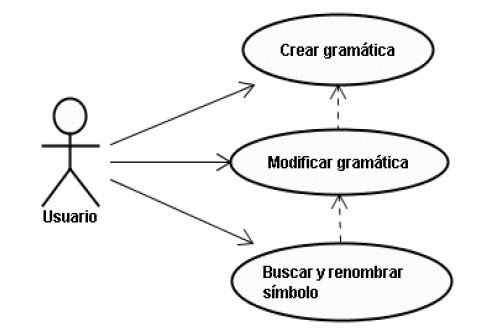
\includegraphics[width=.7\textwidth]{CasoUso-ModificarCrearGramatica}
\caption{Diagrama de caso de uso Crear/Modificar Gramática.\cite{thothv2}}
\label{fig:B.2}
\end{figure}


\begin{table}[]
\centering
\begin{tabular}{@{}
>{\columncolor[HTML]{FFFFFF}}p {.25\textwidth} p {.75\textwidth}@{}}
\toprule
\textbf{Caso de uso 4}   & Crear gramática.                                                                                                                                                                                                                                                                                                                                                          \\ \midrule
\textbf{Versión}         & 1.0                                                                                                                                                                                                                                                                                                                                                                                                                                                                                                                                                                                                                                                                                                                                                                                                 \\ \midrule
\textbf{Personal involucrado}   & Usuario
 \\ \midrule
\textbf{Descripción}     & \begin{tabular}[c]{@{}l@{}}Introducir una gramática\\Los campos de características de la gramática están vacíos.\end{tabular}                                                                                                                                                                                                                           \\ \midrule
\textbf{Precondiciones}  & \begin{tabular}[c]{@{}l@{}}Se debe tener una sesión abierta.\end{tabular}                                                                                                                                                                                                                                                                                                     \\ \midrule
\textbf{Acciones}        & \begin{tabular}[c]{@{}l@{}}1 Acceder al menú principal.\\2 Introducir una gramática \\3 Comprobar dicha gramática.\end{tabular}
\\ \midrule
\textbf{Postcondiciones} & \begin{tabular}[c]{@{}l@{}}La comprobación ha sido correcta y no ha emitido ningún\\ mensaje de error. La tabla características se encuentra\\ completada con los datos.\end{tabular}                                                                                                                                                                                                                                                                                         \\ \midrule
\textbf{Excepciones}     & \begin{tabular}[c]{@{}l@{}}Gramática con sintaxis incorrecta.\end{tabular}
\\ \midrule
\textbf{Frecuencia}     & \begin{tabular}[c]{@{}l@{}}Alta\end{tabular}                                                                                                                                                                                                                                                                                                          \\ \midrule
\textbf{Importancia}     & Alta                                                                                                                                                                                                                                                                                                                                                                                                            \\ \bottomrule
\end{tabular}
\caption{Caso de uso Crear gramática.}
\label{tab:tablacaso4}
\end{table}


\begin{table}[]
\centering
\begin{tabular}{@{}
>{\columncolor[HTML]{FFFFFF}}p {.25\textwidth} p {.75\textwidth}@{}}
\toprule
\textbf{Caso de uso 5}   & Modificar gramática.                                                                                                                                                                                                                                                                                                                                                          \\ \midrule
\textbf{Versión}         & 1.0                                                                                                                                                                                                                                                                                                                                                                                                                                                                                                                                                                                                                                                                                                                                                                                                 \\ \midrule
\textbf{Personal involucrado}   & Usuario
 \\ \midrule
\textbf{Descripción}     & \begin{tabular}[c]{@{}l@{}}Consiste en realizar cambios sobre una gramática ya\\ escrita en el panel.\end{tabular}                                                                                                                                                                                                                           \\ \midrule
\textbf{Precondiciones}  & \begin{tabular}[c]{@{}l@{}}Se debe tener una sesión abierta.\\Debe haber introducido una gramática.\end{tabular}                                                                                                                                                                                                                                                                                                     \\ \midrule
\textbf{Acciones}        & \begin{tabular}[c]{@{}l@{}}1 Introducir una nueva gramática \\3 Comprobar/checkear dicha gramática.\end{tabular}
\\ \midrule
\textbf{Postcondiciones} & \begin{tabular}[c]{@{}l@{}}La comprobación ha sido correcta y no ha emitido ningún\\ mensaje de error.La tabla características se encuentra\\ completada con los datos.\end{tabular}                                                                                                                                                                                                                                                                                         \\ \midrule
\textbf{Excepciones}     & \begin{tabular}[c]{@{}l@{}}Gramática con sintaxis incorrecta.\end{tabular}
\\ \midrule
\textbf{Frecuencia}     & \begin{tabular}[c]{@{}l@{}}Media\end{tabular}                                                                                                                                                                                                                                                                                                          \\ \midrule
\textbf{Importancia}     & Alta                                                                                                                                                                                                                                                                                                                                                                                                            \\ \bottomrule
\end{tabular}
\caption{Caso de uso Modificar gramática.}
\label{tab:tablacaso5}
\end{table}



\begin{table}[]
\centering
\begin{tabular}{@{}
>{\columncolor[HTML]{FFFFFF}}p {.25\textwidth} p {.75\textwidth}@{}}
\toprule
\textbf{Caso de uso 6}   & Buscar y renombrar símbolo.                                                                                                                                                                                                                                                                                                                                                          \\ \midrule
\textbf{Versión}         & 1.0                                                                                                                                                                                                                                                                                                                                                                                                                                                                                                                                                                                                                                                                                                                                                                                                 \\ \midrule
\textbf{Personal involucrado}   & Usuario
 \\ \midrule
\textbf{Descripción}     & \begin{tabular}[c]{@{}l@{}}Una vez se tenga una gramática sustituir algún símbolo\\ de ella por uno nuevo.\end{tabular}                                                                                                                                                                                                                           \\ \midrule
\textbf{Precondiciones}  & \begin{tabular}[c]{@{}l@{}}Se debe tener una sesión abierta.\\Debe haber introducido una gramática.\end{tabular}                                                                                                                                                                                                                                                                                                     \\ \midrule
\textbf{Acciones}        & \begin{tabular}[c]{@{}l@{}}1 Si la gramática esta comprobada pasa a 4.\\2 Si la gramática no esta comprobada pasa a 3.\\3 Comprobar/checkear dicha gramática.\\4 Busca el símbolo introducido \\5 Sustituye el símbolo por otro nuevo introducido por el\\ usuario.\end{tabular}
\\ \midrule
\textbf{Postcondiciones} & \begin{tabular}[c]{@{}l@{}}Aparece una gramática nueva con las sustituciones.\end{tabular}                                                                                                                                                                                                                                                                                         \\ \midrule
\textbf{Excepciones}     & \begin{tabular}[c]{@{}l@{}}Gramática con sintaxis incorrecta.\\El usuario no pulsa en aceptar\\El símbolo a sustituir no existe.\end{tabular}
\\ \midrule
\textbf{Frecuencia}     & \begin{tabular}[c]{@{}l@{}}Baja\end{tabular}                                                                                                                                                                                                                                                                                                          \\ \midrule
\textbf{Importancia}     & Alta                                                                                                                                                                                                                                                                                                                                                                                                            \\ \bottomrule
\end{tabular}
\caption{Caso de uso Buscar y renombrar símbolo.}
\label{tab:tablacaso6}
\end{table}

\begin{figure}[h]
\centering
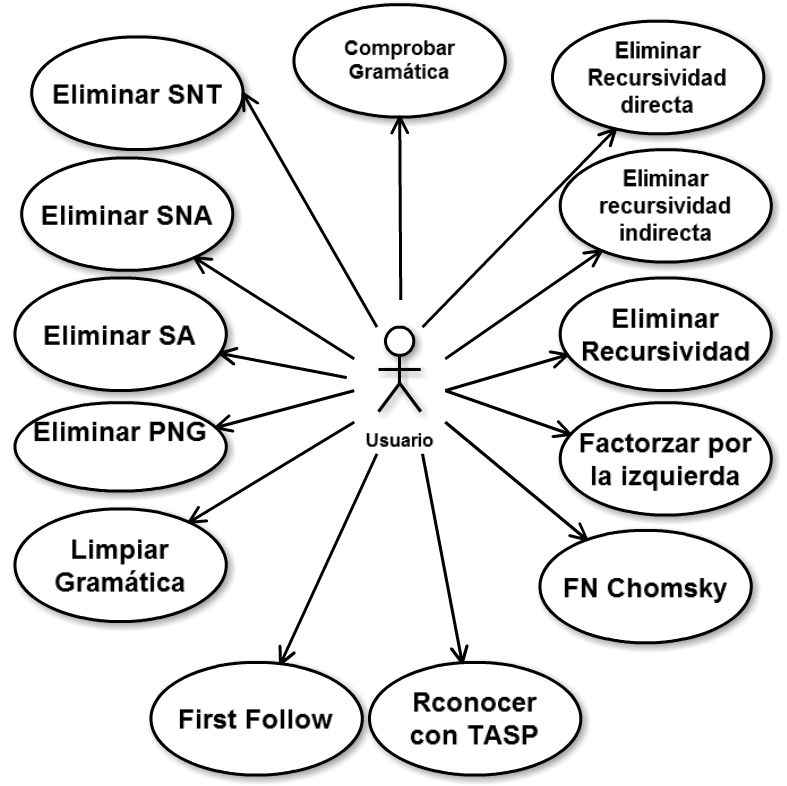
\includegraphics[width=.7\textwidth]{CasoUso-Algoritmos}
\caption{Diagrama de caso de uso Algoritmos.}
\label{fig:B.3}
\end{figure}


\begin{table}[]
\centering
\begin{tabular}{@{}
>{\columncolor[HTML]{FFFFFF}}p {.25\textwidth} p {.75\textwidth}@{}}
\toprule
\textbf{Caso de uso 7}   & Realizar algoritmos.                                                                                                                                                                                                                                                                                                                                                          \\ \midrule
\textbf{Versión}         & 1.0                                                                                                                                                                                                                                                                                                                                                                                                                                                                                                                                                                                                                                                                                                                                                                                                 \\ \midrule
\textbf{Personal involucrado}   & Usuario
 \\ \midrule
\textbf{Descripción}     & \begin{tabular}[c]{@{}l@{}}Se limpia la ventana y aparece una vista con el algoritmo.\end{tabular}                                                                                                                                                                                                                           \\ \midrule
\textbf{Precondiciones}  & \begin{tabular}[c]{@{}l@{}}Se debe tener una sesión abierta.\\Debe haber creado una gramática.\\Haber comprobado la gramática.\end{tabular}                                                                                                                                                                                                                                                                                                     \\ \midrule
\textbf{Acciones}        & \begin{tabular}[c]{@{}l@{}}1 El usuario pincha en el menú en algoritmos.\\2 Aparece un desplegable con todos los algoritmos.\end{tabular}
\\ \midrule
\textbf{Postcondiciones} & \begin{tabular}[c]{@{}l@{}}Aparece una nueva vista con los paneles del algoritmo.\end{tabular}                                                                                                                                                                                                                                                                                         \\ \midrule
\textbf{Excepciones}     & \begin{tabular}[c]{@{}l@{}}Gramática con sintaxis incorrecta.\\El usuario no ha comprobado la gramática\end{tabular}
\\ \midrule
\textbf{Frecuencia}     & \begin{tabular}[c]{@{}l@{}}Alta\end{tabular}                                                                                                                                                                                                                                                                                                          \\ \midrule
\textbf{Importancia}     & Alta                                                                                                                                                                                                                                                                                                                                                                                                            \\ \bottomrule
\end{tabular}
\caption{Caso de uso de algoritmos.}
\label{tab:tablacaso7}
\end{table}

\begin{table}[]
\centering
\begin{tabular}{@{}
>{\columncolor[HTML]{FFFFFF}}p {.25\textwidth} p {.75\textwidth}@{}}
\toprule
\textbf{Caso de uso 8}   & Eliminar símbolos no terminables.                                                                                                                                                                                                                                                                                                                                                          \\ \midrule
\textbf{Versión}         & 1.0                                                                                                                                                                                                                                                                                                                                                                                                                                                                                                                                                                                                                                                                                                                                                                                                 \\ \midrule
\textbf{Personal involucrado}   & Usuario
 \\ \midrule
\textbf{Descripción}     & \begin{tabular}[c]{@{}l@{}}Se eliminan aquellos símbolos que no sean terminables, \\que sean de paso, de la gramática.\end{tabular}                                                                                                                                                                                                                           \\ \midrule
\textbf{Precondiciones}  & \begin{tabular}[c]{@{}l@{}}Se debe tener una sesión abierta.\\Debe haber creado una gramática.\\Haber comprobado la gramática.\end{tabular}                                                                                                                                                                                                                                                                                                     \\ \midrule
\textbf{Acciones}        & \begin{tabular}[c]{@{}l@{}}1. El usuario selecciona eliminar símbolos no\\terminables. \\2. Se crea una vista de la gramática y de la nueva gramá-\\tica en la que se van a realizar los pasos del algoritmo\\eliminación de símbolos no terminables.\\3. El usuario puede:\\3.1.Pulsar sobre siguiente paso hasta que se\\llegue al final del algoritmo.\\3.2.Pulsar sobre todos los pasos.\\4. El usuario pulsa sobre aceptar.\end{tabular}
\\ \midrule
\textbf{Postcondiciones} & \begin{tabular}[c]{@{}l@{}}Aparece una nueva vista en el menú con la gramática\\resultante.\end{tabular}                                                                                                                                                                                                                                                                                         \\ \midrule
\textbf{Excepciones}     & \begin{tabular}[c]{@{}l@{}}Gramática con sintaxis incorrecta.\\El usuario pulsa cancelar\end{tabular}
\\ \midrule
\textbf{Frecuencia}     & \begin{tabular}[c]{@{}l@{}}Media\end{tabular}                                                                                                                                                                                                                                                                                                          \\ \midrule
\textbf{Importancia}     & Alta                                                                                                                                                                                                                                                                                                                                                                                                            \\ \bottomrule
\end{tabular}
\caption{Caso de uso de Eliminar símbolos no terminables.}
\label{tab:tablacaso8}
\end{table}

\begin{table}[]
\centering
\begin{tabular}{@{}
>{\columncolor[HTML]{FFFFFF}}p {.25\textwidth} p {.75\textwidth}@{}}
\toprule
\textbf{Caso de uso 9}   & Eliminar símbolos no alcanzables.                                                                                                                                                                                                                                                                                                                                                          \\ \midrule
\textbf{Versión}         & 1.0                                                                                                                                                                                                                                                                                                                                                                                                                                                                                                                                                                                                                                                                                                                                                                                                 \\ \midrule
\textbf{Personal involucrado}   & Usuario
 \\ \midrule
\textbf{Descripción}     & \begin{tabular}[c]{@{}l@{}}Se eliminan aquellos símbolos que no sean alcanzables\end{tabular}                                                                                                                                                                                                                           \\ \midrule
\textbf{Precondiciones}  & \begin{tabular}[c]{@{}l@{}}Se debe tener una sesión abierta.\\Debe haber creado una gramática.\\Haber comprobado la gramática.\end{tabular}                                                                                                                                                                                                                                                                                                     \\ \midrule
\textbf{Acciones}        & \begin{tabular}[c]{@{}l@{}}1. El usuario selecciona eliminar símbolos no\\alcanzables. \\2. Se crea una vista de la gramática y de la nueva gramá-\\tica en la que se van a realizar los pasos del algoritmo\\eliminación de símbolos no alcanzables.\\3. El usuario puede:\\3.1.Pulsar sobre siguiente paso hasta que se\\llegue al final del algoritmo.\\3.2.Pulsar sobre todos los pasos.\\4. El usuario pulsa sobre aceptar.\end{tabular}
\\ \midrule
\textbf{Postcondiciones} & \begin{tabular}[c]{@{}l@{}}Aparece una nueva vista en el menú con la gramática \\resultante.\end{tabular}                                                                                                                                                                                                                                                                                         \\ \midrule
\textbf{Excepciones}     & \begin{tabular}[c]{@{}l@{}}Gramática con sintaxis incorrecta.\\El usuario pulsa cancelar\end{tabular}
\\ \midrule
\textbf{Frecuencia}     & \begin{tabular}[c]{@{}l@{}}Media\end{tabular}                                                                                                                                                                                                                                                                                                          \\ \midrule
\textbf{Importancia}     & Alta                                                                                                                                                                                                                                                                                                                                                                                                            \\ \bottomrule
\end{tabular}
\caption{Caso de uso de Eliminar símbolos no alcanzables.}
\label{tab:tablacaso9}
\end{table}


\begin{table}[]
\centering
\begin{tabular}{@{}
>{\columncolor[HTML]{FFFFFF}}p {.25\textwidth} p {.75\textwidth}@{}}
\toprule
\textbf{Caso de uso 10}   & Eliminar símbolos anulables.                                                                                                                                                                                                                                                                                                                                                          \\ \midrule
\textbf{Versión}         & 1.0                                                                                                                                                                                                                                                                                                                                                                                                                                                                                                                                                                                                                                                                                                                                                                                                 \\ \midrule
\textbf{Personal involucrado}   & Usuario
 \\ \midrule
\textbf{Descripción}     & \begin{tabular}[c]{@{}l@{}}Se Eliminan aquellos símbolos que sean terminables\end{tabular}                                                                                                                                                                                                                           \\ \midrule
\textbf{Precondiciones}  & \begin{tabular}[c]{@{}l@{}}Se debe tener una sesión abierta.\\Debe haber creado una gramática.\\Haber comprobado la gramática.\end{tabular}                                                                                                                                                                                                                                                                                                     \\ \midrule
\textbf{Acciones}        & \begin{tabular}[c]{@{}l@{}}1. El usuario selecciona eliminar símbolos \\anulables. \\2. Se comprueba que haya producciones
epsilon.\\2.1.Si no hay producciones epsilon, se
abre un warning.\\2.2.Si hay, abre una ventana con la vista de la
gramática\\y de la nueva gramática y en la\\que se van a realizar los pasos del algoritmo\\eliminación de símbolos no terminables.\\3 El usuario puede \\3.1.Pulsar sobre siguiente paso hasta que se\\llegue al final del algoritmo.\\3.2.Pulsar sobre todos los pasos.\\4. El usuario pulsa sobre aceptar.\end{tabular}
\\ \midrule
\textbf{Postcondiciones} & \begin{tabular}[c]{@{}l@{}}Aparece una nueva vista en el menú con la gramática\\ resultante.\end{tabular}                                                                                                                                                                                                                                                                                         \\ \midrule
\textbf{Excepciones}     & \begin{tabular}[c]{@{}l@{}}Gramática con sintaxis incorrecta.\\El usuario pulsa cancelar\\La gramática no tiene producciones epsilon.\end{tabular}
\\ \midrule
\textbf{Frecuencia}     & \begin{tabular}[c]{@{}l@{}}Media\end{tabular}                                                                                                                                                                                                                                                                                                          \\ \midrule
\textbf{Importancia}     & Alta                                                                                                                                                                                                                                                                                                                                                                                                            \\ \bottomrule
\end{tabular}
\caption{Caso de uso de Eliminar símbolos anulables.}
\label{tab:tablacaso10}
\end{table}



\begin{table}[]
\centering
\begin{tabular}{@{}
>{\columncolor[HTML]{FFFFFF}}p {.25\textwidth} p {.75\textwidth}@{}}
\toprule
\textbf{Caso de uso 11}   & Eliminar producciones no generativas.                                                                                                                                                                                                                                                                                                                                                          \\ \midrule
\textbf{Versión}         & 1.0                                                                                                                                                                                                                                                                                                                                                                                                                                                                                                                                                                                                                                                                                                                                                                                                 \\ \midrule
\textbf{Personal involucrado}   & Usuario
 \\ \midrule
\textbf{Descripción}     & \begin{tabular}[c]{@{}l@{}}Se eliminan aquellas producciones que no sean generativas.\end{tabular}                                                                                                                                                                                                                           \\ \midrule
\textbf{Precondiciones}  & \begin{tabular}[c]{@{}l@{}}Se debe tener una sesión abierta.\\Debe haber creado una gramática.\\Haber comprobado la gramática.\end{tabular}                                                                                                                                                                                                                                                                                                     \\ \midrule
\textbf{Acciones}        & \begin{tabular}[c]{@{}l@{}}1. El usuario selecciona eliminar producciones no\\generativas. \\2. Se abre una vista con la gramática y  la nueva gramática\\ y en la que se van a realizar los pasos del\\ algoritmo\\3. El usuario puede:\\3.1.Pulsar sobre siguiente paso hasta que se\\llegue al final del algoritmo.\\3.2.Pulsar sobre todos los pasos.\\4. El usuario pulsa sobre aceptar.\end{tabular}
\\ \midrule
\textbf{Postcondiciones} & \begin{tabular}[c]{@{}l@{}}Aparece una nueva vista en el menú con la gramática\\resultante.\end{tabular}                                                                                                                                                                                                                                                                                         \\ \midrule
\textbf{Excepciones}     & \begin{tabular}[c]{@{}l@{}}Gramática con sintaxis incorrecta.\\El usuario pulsa cancelar\end{tabular}
\\ \midrule
\textbf{Frecuencia}     & \begin{tabular}[c]{@{}l@{}}Media\end{tabular}                                                                                                                                                                                                                                                                                                          \\ \midrule
\textbf{Importancia}     & Alta                                                                                                                                                                                                                                                                                                                                                                                                            \\ \bottomrule
\end{tabular}
\caption{Caso de uso de Eliminar producciones no generativas.}
\label{tab:tablacaso11}
\end{table}


\begin{table}[]
\centering
\begin{tabular}{@{}
>{\columncolor[HTML]{FFFFFF}}p {.25\textwidth} p {.75\textwidth}@{}}
\toprule
\textbf{Caso de uso 12}   & Limpiar gramática.                                                                                                                                                                                                                                                                                                                                                          \\ \midrule
\textbf{Versión}         & 1.0                                                                                                                                                                                                                                                                                                                                                                                                                                                                                                                                                                                                                                                                                                                                                                                                 \\ \midrule
\textbf{Personal involucrado}   & Usuario
 \\ \midrule
\textbf{Descripción}     & \begin{tabular}[c]{@{}l@{}}Se eliminan: símbolos no terminables, no alcanzables,\\ anulables y producciones no generativas.\end{tabular}                                                                                                                                                                                                                           \\ \midrule
\textbf{Precondiciones}  & \begin{tabular}[c]{@{}l@{}}Se debe tener una sesión abierta.\\Debe haber creado una gramática.\\Haber comprobado la gramática.\end{tabular}                                                                                                                                                                                                                                                                                                     \\ \midrule
\textbf{Acciones}        & \begin{tabular}[c]{@{}l@{}}1. El usuario selecciona limpiar gramática\\2.1. Si no es necesario limpiar la gramática\\ se indicará en un mensaje de error\\2.2 Realiza la limpieza de forma normal\end{tabular}
\\ \midrule
\textbf{Postcondiciones} & \begin{tabular}[c]{@{}l@{}}Aparece la gramática ya limpia.\end{tabular}                                                                                                                                                                                                                                                                                         \\ \midrule
\textbf{Excepciones}     & \begin{tabular}[c]{@{}l@{}}Gramática con sintaxis incorrecta.\\No es necesario limpiar la gramática\end{tabular}
\\ \midrule
\textbf{Frecuencia}     & \begin{tabular}[c]{@{}l@{}}Media\end{tabular}                                                                                                                                                                                                                                                                                                          \\ \midrule
\textbf{Importancia}     & Alta                                                                                                                                                                                                                                                                                                                                                                                                            \\ \bottomrule
\end{tabular}
\caption{Caso de uso de Limpiar gramática.}
\label{tab:tablacaso12}
\end{table}


\begin{table}[]
\centering
\begin{tabular}{@{}
>{\columncolor[HTML]{FFFFFF}}p {.25\textwidth} p {.75\textwidth}@{}}
\toprule
\textbf{Caso de uso 13}   & Eliminar recursividad directa.                                                                                                                                                                                                                                                                                                                                                          \\ \midrule
\textbf{Versión}         & 1.0                                                                                                                                                                                                                                                                                                                                                                                                                                                                                                                                                                                                                                                                                                                                                                                                 \\ \midrule
\textbf{Personal involucrado}   & Usuario
 \\ \midrule
\textbf{Descripción}     & \begin{tabular}[c]{@{}l@{}}Se encarga de la eliminación de la recursividad\\ directa de una gramática\end{tabular}                                                                                                                                                                                                                           \\ \midrule
\textbf{Precondiciones}  & \begin{tabular}[c]{@{}l@{}}Se debe tener una sesión abierta.\\Debe haber creado una gramática.\\Haber comprobado la gramática.\end{tabular}                                                                                                                                                                                                                                                                                                     \\ \midrule
\textbf{Acciones}        & \begin{tabular}[c]{@{}l@{}}1. El usuario selecciona eliminar recursividad\\directa\\2. Se abre una vista de la gramática y de la nueva gramática\\ y en la que se van a realizar los pasos del algoritmo eliminación de recursividad directa:\\3. El usuario puede:\\
3.1.Pulsar sobre siguiente paso hasta que se\\llegue al final del algoritmo.\\
3.2.Pulsar sobre todos los pasos.\\4. El usuario pulsa sobre aceptar.\end{tabular}
\\ \midrule
\textbf{Postcondiciones} & \begin{tabular}[c]{@{}l@{}}Aparece la gramática sin recursividad directa.\end{tabular}                                                                                                                                                                                                                                                                                         \\ \midrule
\textbf{Excepciones}     & \begin{tabular}[c]{@{}l@{}}Gramática con sintaxis incorrecta.\\El usuario pulsa cancelar.\\La gramática no tiene recursividad directa\end{tabular}
\\ \midrule
\textbf{Frecuencia}     & \begin{tabular}[c]{@{}l@{}}Media\end{tabular}                                                                                                                                                                                                                                                                                                          \\ \midrule
\textbf{Importancia}     & Alta                                                                                                                                                                                                                                                                                                                                                                                                            \\ \bottomrule
\end{tabular}
\caption{Caso de uso de Eliminar recursividad directa.}
\label{tab:tablacaso13}
\end{table}


\begin{table}[]
\centering
\begin{tabular}{@{}
>{\columncolor[HTML]{FFFFFF}}p {.25\textwidth} p {.75\textwidth}@{}}
\toprule
\textbf{Caso de uso 14}   & Eliminar recursividad indirecta.                                                                                                                                                                                                                                                                                                                                                          \\ \midrule
\textbf{Versión}         & 1.0                                                                                                                                                                                                                                                                                                                                                                                                                                                                                                                                                                                                                                                                                                                                                                                                 \\ \midrule
\textbf{Personal involucrado}   & Usuario
 \\ \midrule
\textbf{Descripción}     & \begin{tabular}[c]{@{}l@{}}Se encarga de la eliminación de la recursividad\\indirecta de una gramática\end{tabular}                                                                                                                                                                                                                           \\ \midrule
\textbf{Precondiciones}  & \begin{tabular}[c]{@{}l@{}}Se debe tener una sesión abierta.\\Debe haber creado una gramática.\\Haber comprobado la gramática.\end{tabular}                                                                                                                                                                                                                                                                                                     \\ \midrule
\textbf{Acciones}        & \begin{tabular}[c]{@{}l@{}}1. El usuario selecciona eliminar recursividad\\indirecta\\2. Se abre una vista de la gramática y de la nueva gramática\\ y en la que se van a realizar los pasos del algoritmo eliminación de recursividad indirecta:\\3. El usuario puede:\\
3.1.Pulsar sobre siguiente paso hasta que se\\llegue al final del algoritmo.\\
3.2.Pulsar sobre todos los pasos.\\4. El usuario pulsa sobre aceptar.\end{tabular}
\\ \midrule
\textbf{Postcondiciones} & \begin{tabular}[c]{@{}l@{}}Aparece gramática sin recursividad indirecta.\end{tabular}                                                                                                                                                                                                                                                                                         \\ \midrule
\textbf{Excepciones}     & \begin{tabular}[c]{@{}l@{}}Gramática con sintaxis incorrecta.\\El usuario pulsa cancelar.\\La gramática no tiene recursividad indirecta\end{tabular}
\\ \midrule
\textbf{Frecuencia}     & \begin{tabular}[c]{@{}l@{}}Media\end{tabular}                                                                                                                                                                                                                                                                                                          \\ \midrule
\textbf{Importancia}     & Alta                                                                                                                                                                                                                                                                                                                                                                                                            \\ \bottomrule
\end{tabular}
\caption{Caso de uso de Eliminar recursividad indirecta.}
\label{tab:tablacaso14}
\end{table}


\begin{table}[]
\centering
\begin{tabular}{@{}
>{\columncolor[HTML]{FFFFFF}}p {.25\textwidth} p {.75\textwidth}@{}}
\toprule
\textbf{Caso de uso 15}   & Eliminar recursividad.                                                                                                                                                                                                                                                                                                                                                          \\ \midrule
\textbf{Versión}         & 1.0                                                                                                                                                                                                                                                                                                                                                                                                                                                                                                                                                                                                                                                                                                                                                                                                 \\ \midrule
\textbf{Personal involucrado}   & Usuario
 \\ \midrule
\textbf{Descripción}     & \begin{tabular}[c]{@{}l@{}}Elimina la recursividad de la gramática, tanto la directa\\así como la indirecta.\end{tabular}                                                                                                                                                                                                                           \\ \midrule
\textbf{Precondiciones}  & \begin{tabular}[c]{@{}l@{}}Se debe tener una sesión abierta.\\Debe haber creado una gramática.\\Haber comprobado la gramática.\end{tabular}                                                                                                                                                                                                                                                                                                     \\ \midrule
\textbf{Acciones}        & \begin{tabular}[c]{@{}l@{}}1. El usuario selecciona eliminar recursividad\\2. Se realiza los algoritmos:\\2.1. Eliminar recursividad directa.\\2.2. Eliminar recursividad indirecta\\3.1. Si no hay recursividad directa ni indirecta aparece un\\ mensaje de error.\\3.2. En el área de texto aparece la gramática sin recursividad.\end{tabular}
\\ \midrule
\textbf{Postcondiciones} & \begin{tabular}[c]{@{}l@{}}Aparece la gramática sin recursividad.\end{tabular}                                                                                                                                                                                                                                                                                         \\ \midrule
\textbf{Excepciones}     & \begin{tabular}[c]{@{}l@{}}Gramática con sintaxis incorrecta.\\El usuario pulsa cancelar.\\La gramática no tiene recursividad directa ni indirecta\end{tabular}
\\ \midrule
\textbf{Frecuencia}     & \begin{tabular}[c]{@{}l@{}}Media\end{tabular}                                                                                                                                                                                                                                                                                                          \\ \midrule
\textbf{Importancia}     & Alta                                                                                                                                                                                                                                                                                                                                                                                                            \\ \bottomrule
\end{tabular}
\caption{Caso de uso de Eliminar recursividad.}
\label{tab:tablacaso15}
\end{table}


\begin{table}[]
\centering
\begin{tabular}{@{}
>{\columncolor[HTML]{FFFFFF}}p {.25\textwidth} p {.75\textwidth}@{}}
\toprule
\textbf{Caso de uso 16}   & Factorizar por la izquierda.                                                                                                                                                                                                                                                                                                                                                          \\ \midrule
\textbf{Versión}         & 1.0                                                                                                                                                                                                                                                                                                                                                                                                                                                                                                                                                                                                                                                                                                                                                                                                 \\ \midrule
\textbf{Personal involucrado}   & Usuario
 \\ \midrule
\textbf{Descripción}     & \begin{tabular}[c]{@{}l@{}}Se encarga de factorizar la gramática\\ que se le pasa.\end{tabular}                                                                                                                                                                                                                           \\ \midrule
\textbf{Precondiciones}  & \begin{tabular}[c]{@{}l@{}}Se debe tener una sesión abierta.\\Debe haber creado una gramática.\\Haber comprobado la gramática.\end{tabular}                                                                                                                                                                                                                                                                                                     \\ \midrule
\textbf{Acciones}        & \begin{tabular}[c]{@{}l@{}}1. El usuario selecciona factorizar por la izquierda\\2. Se abre una vista de la gramática y de la nueva gramática\\ y en la que se van a realizar los pasos del algoritmo\\3. El usuario puede:\\
3.1.Pulsar sobre siguiente paso hasta que se\\llegue al final del algoritmo.\\
3.2.Pulsar sobre todos los pasos.\\4. El usuario pulsa sobre aceptar.\end{tabular}
\\ \midrule
\textbf{Postcondiciones} & \begin{tabular}[c]{@{}l@{}}Aparece una vista con la  gramática factorizada.\end{tabular}                                                                                                                                                                                                                                                                                         \\ \midrule
\textbf{Excepciones}     & \begin{tabular}[c]{@{}l@{}}Gramática con sintaxis incorrecta.\\El usuario pulsa cancelar.\end{tabular}
\\ \midrule
\textbf{Frecuencia}     & \begin{tabular}[c]{@{}l@{}}Media\end{tabular}                                                                                                                                                                                                                                                                                                          \\ \midrule
\textbf{Importancia}     & Alta                                                                                                                                                                                                                                                                                                                                                                                                            \\ \bottomrule
\end{tabular}
\caption{Caso de uso de Factorizar por la izquierda.}
\label{tab:tablacaso16}
\end{table}


\begin{table}[]
\centering
\begin{tabular}{@{}
>{\columncolor[HTML]{FFFFFF}}p {.25\textwidth} p {.75\textwidth}@{}}
\toprule
\textbf{Caso de uso 17}   & Forma normal de Chomsky.                                                                                                                                                                                                                                                                                                                                                          \\ \midrule
\textbf{Versión}         & 1.0                                                                                                                                                                                                                                                                                                                                                                                                                                                                                                                                                                                                                                                                                                                                                                                                 \\ \midrule
\textbf{Personal involucrado}   & Usuario
 \\ \midrule
\textbf{Descripción}     & \begin{tabular}[c]{@{}l@{}}Transforma la gramática a forma normal de Chomsky.\end{tabular}                                                                                                                                                                                                                           \\ \midrule
\textbf{Precondiciones}  & \begin{tabular}[c]{@{}l@{}}Se debe tener una sesión abierta.\\Debe haber creado una gramática.\\Haber comprobado la gramática.\end{tabular}                                                                                                                                                                                                                                                                                                     \\ \midrule
\textbf{Acciones}        & \begin{tabular}[c]{@{}l@{}}1. El usuario selecciona forma normal de Chomsky\\2. Se abre una vista de la gramática y de la nueva gramática\\y en la que se van a realizar los pasos del algoritmo\\3. El usuario puede:\\
3.1.Pulsar sobre siguiente paso hasta que se\\llegue al final del algoritmo.\\
3.2.Pulsar sobre todos los pasos.\\4. El usuario pulsa sobre aceptar.\end{tabular}
\\ \midrule
\textbf{Postcondiciones} & \begin{tabular}[c]{@{}l@{}}Aparece una vista con la nueva la gramática.\end{tabular}                                                                                                                                                                                                                                                                                         \\ \midrule
\textbf{Excepciones}     & \begin{tabular}[c]{@{}l@{}}Gramática con sintaxis incorrecta.\\El usuario pulsa cancelar.\end{tabular}
\\ \midrule
\textbf{Frecuencia}     & \begin{tabular}[c]{@{}l@{}}Media\end{tabular}                                                                                                                                                                                                                                                                                                          \\ \midrule
\textbf{Importancia}     & Alta                                                                                                                                                                                                                                                                                                                                                                                                            \\ \bottomrule
\end{tabular}
\caption{Caso de uso de Forma normal de Chomsky.}
\label{tab:tablacaso17}
\end{table}



\begin{table}[]
\centering
\begin{tabular}{@{}
>{\columncolor[HTML]{FFFFFF}}p {.25\textwidth} p {.75\textwidth}@{}}
\toprule
\textbf{Caso de uso 18}   & Calcular el First y el Follow.                                                                                                                                                                                                                                                                                                                                                          \\ \midrule
\textbf{Versión}         & 1.0                                                                                                                                                                                                                                                                                                                                                                                                                                                                                                                                                                                                                                                                                                                                                                                                 \\ \midrule
\textbf{Personal involucrado}   & Usuario
 \\ \midrule
\textbf{Descripción}     & \begin{tabular}[c]{@{}l@{}}Calcula el first y el follow de cada uno\\de los no terminales de la gramática.\end{tabular}                                                                                                                                                                                                                           \\ \midrule
\textbf{Precondiciones}  & \begin{tabular}[c]{@{}l@{}}Se debe tener una sesión abierta.\\Debe haber creado una gramática.\\Haber comprobado la gramática.\end{tabular}                                                                                                                                                                                                                                                                                                     \\ \midrule
\textbf{Acciones}        & \begin{tabular}[c]{@{}l@{}}1. El usuario selecciona cálculo de  First y Follow.\\2. Se abre una ventana emergente que pregunta si se desea\\continuar.\\3. Si el usuario pulsa en <<si>> se abre una vista de la gramática\\y de la nueva gramática y en la que se van a realizar los pasos del algoritmo\\4. El usuario puede:\\
\\a) Pulsar sobre el botón de first
\\El sistema muestra el calculo de first.
\\b) Pulsar sobre el botón de follow
\\El sistema muestra el follow.
\\c) Pulsar sobre el botón de TASP
\\El sistema realiza el análisis\\descendente por reconocimiento con\\TASP.\end{tabular}
\\ \midrule
\textbf{Postcondiciones} & \begin{tabular}[c]{@{}l@{}}Aparece una vista con la nueva la gramática.\end{tabular}                                                                                                                                                                                                                                                                                         \\ \midrule
\textbf{Excepciones}     & \begin{tabular}[c]{@{}l@{}}Gramática con sintaxis incorrecta.\\El usuario pulsa cancelar.\\El usuario pulsa <<no>>.\end{tabular}
\\ \midrule
\textbf{Frecuencia}     & \begin{tabular}[c]{@{}l@{}}Media\end{tabular}                                                                                                                                                                                                                                                                                                          \\ \midrule
\textbf{Importancia}     & Alta                                                                                                                                                                                                                                                                                                                                                                                                            \\ \bottomrule
\end{tabular}
\caption{Caso de uso de First y follow.}
\label{tab:tablacaso18}
\end{table}


\begin{table}[]
\centering
\begin{tabular}{@{}
>{\columncolor[HTML]{FFFFFF}}p {.25\textwidth} p {.75\textwidth}@{}}
\toprule
\textbf{Caso de uso 19}   & Reconocimiento con TASP.                                                                                                                                                                                                                                                                                                                                                          \\ \midrule
\textbf{Versión}         & 1.0                                                                                                                                                                                                                                                                                                                                                                                                                                                                                                                                                                                                                                                                                                                                                                                                 \\ \midrule
\textbf{Personal involucrado}   & Usuario
 \\ \midrule
\textbf{Descripción}     & \begin{tabular}[c]{@{}l@{}}Introducir una palabra
para que sea reconocida\\por el autómata de pila que representa la TASP.\end{tabular}                                                                                                                                                                                                                           \\ \midrule
\textbf{Precondiciones}  & \begin{tabular}[c]{@{}l@{}}Se debe tener una sesión abierta.\\Debe haber creado una gramática.\\Haber comprobado la gramática.\end{tabular}                                                                                                                                                                                                                                                                                                     \\ \midrule
\textbf{Acciones}        & \begin{tabular}[c]{@{}l@{}}1. El usuario selecciona reconocimiento con TASP.\\2. Se abre una ventana emergente que pregunta si se desea\\continuar.\\3. Si el usuario pulsa en <<si>> se abre una vista de la gramática\\ y de la nueva gramática y en la que se van a realizar los pasos del algoritmo\\4. El usuario puede Introducir una palabra y:
\\a) Pulsar sobre siguiente paso hasta que se\\llegue al final del análisis.
\\b) Pulsar sobre todos los pasos para que lo haga directamente 
\\c) Pulsar en borrar palabra y volver a paso 4.
\\5. Se mostrará si la palabra ha sido reconocida o no.\end{tabular}
\\ \midrule
\textbf{Postcondiciones} & \begin{tabular}[c]{@{}l@{}}Mensaje de palabra reconocida o no reconocida. \end{tabular}                                                                                                                                                                                                                                                                                         \\ \midrule
\textbf{Excepciones}     & \begin{tabular}[c]{@{}l@{}}Gramática con sintaxis incorrecta.\\El usuario pulsa cancelar.\\El usuario pulsa <<no>>.\end{tabular}
\\ \midrule
\textbf{Frecuencia}     & \begin{tabular}[c]{@{}l@{}}Media\end{tabular}                                                                                                                                                                                                                                                                                                          \\ \midrule
\textbf{Importancia}     & Alta                                                                                                                                                                                                                                                                                                                                                                                                            \\ \bottomrule
\end{tabular}
\caption{Caso de uso de Reconocimiento con TASP.}
\label{tab:tablacaso19}
\end{table}


\begin{figure}[h]
\centering
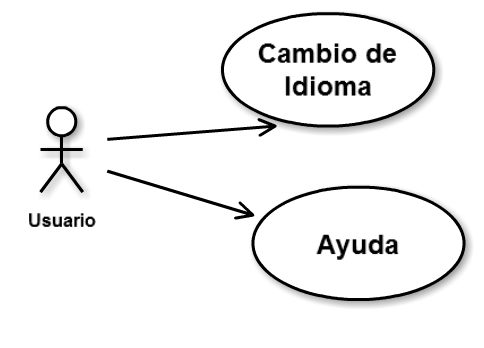
\includegraphics[width=.7\textwidth]{CasoUso-Opciones}
\caption{Diagrama de caso de uso Opciones.}
\label{fig:B.4}
\end{figure}


\begin{table}[]
\centering
\begin{tabular}{@{}
>{\columncolor[HTML]{FFFFFF}}p {.25\textwidth} p {.75\textwidth}@{}}
\toprule
\textbf{Caso de uso 20}   & Cambiar idiomas.                                                                                                                                                                                                                                                                                                                                                          \\ \midrule
\textbf{Versión}         & 1.0                                                                                                                                                                                                                                                                                                                                                                                                                                                                                                                                                                                                                                                                                                                                                                                                 \\ \midrule
\textbf{Personal involucrado}   & Usuario
 \\ \midrule
\textbf{Descripción}     & \begin{tabular}[c]{@{}l@{}}Elegir el idioma en el que se quiere mostrar los textos de\\la aplicación\end{tabular}                                                                                                                                                                                                                           \\ \midrule
\textbf{Precondiciones}  & \begin{tabular}[c]{@{}l@{}}Se debe tener una sesión abierta.\end{tabular}                                                                                                                                                                                                                                                                                                     \\ \midrule
\textbf{Acciones}        & \begin{tabular}[c]{@{}l@{}}1. El usuario selecciona idioma en el menú.\\2. El usuario elige el idioma\\3. Se abre una ventana emergente que pregunta si se desea\\continuar.\\3.1. Si el usuario pulsa en <<si>> se reinicia la vista\\3.2. El usuario pulsa <<no>> la ventana emergente desaparece\\sin hacer nada.\end{tabular}
\\ \midrule
\textbf{Postcondiciones} & \begin{tabular}[c]{@{}l@{}}Los textos se muestran en el idioma elegido. \end{tabular}                                                                                                                                                                                                                                                                                         \\ \midrule
\textbf{Excepciones}     & \begin{tabular}[c]{@{}l@{}}.\\El usuario pulsa <<no>> en la ventana emergente.\end{tabular}
\\ \midrule
\textbf{Frecuencia}     & \begin{tabular}[c]{@{}l@{}}Baja\end{tabular}                                                                                                                                                                                                                                                                                                          \\ \midrule
\textbf{Importancia}     & Alta                                                                                                                                                                                                                                                                                                                                                                                                            \\ \bottomrule
\end{tabular}
\caption{Caso de uso de Cambio de idioma.}
\label{tab:tablacaso20}
\end{table}

\begin{table}[]
\centering
\begin{tabular}{@{}
>{\columncolor[HTML]{FFFFFF}}p {.25\textwidth} p {.75\textwidth}@{}}
\toprule
\textbf{Caso de uso 21}   & Mostrar Acerca de.                                                                                                                                                                                                                                                                                                                                                          \\ \midrule
\textbf{Versión}         & 1.0                                                                                                                                                                                                                                                                                                                                                                                                                                                                                                                                                                                                                                                                                                                                                                                                 \\ \midrule
\textbf{Personal involucrado}   & Usuario
 \\ \midrule
\textbf{Descripción}     & \begin{tabular}[c]{@{}l@{}}Se muestra información detallada de la aplicación.\end{tabular}                                                                                                                                                                                                                           \\ \midrule
\textbf{Precondiciones}  & \begin{tabular}[c]{@{}l@{}}Se debe tener una sesión abierta.\end{tabular}                                                                                                                                                                                                                                                                                                     \\ \midrule
\textbf{Acciones}        & \begin{tabular}[c]{@{}l@{}}1. El usuario selecciona ayuda en el menú.\\2. El usuario elige la opción Acerca de.\end{tabular}
\\ \midrule
\textbf{Postcondiciones} & \begin{tabular}[c]{@{}l@{}}Se muestra información sobre la aplicación.\end{tabular}                                                                                                                                                                                                                                                                                         \\ \midrule
\textbf{Excepciones}     & 
\\ \midrule
\textbf{Frecuencia}     & \begin{tabular}[c]{@{}l@{}}Baja\end{tabular}                                                                                                                                                                                                                                                                                                          \\ \midrule
\textbf{Importancia}     & Alta                                                                                                                                                                                                                                                                                                                                                                                                            \\ \bottomrule
\end{tabular}
\caption{Caso de uso de Mostrar Acerca de.}
\label{tab:tablacaso21}
\end{table}
